\documentclass[11pt]{book}
\usepackage[T1]{fontenc}
\usepackage[utf8]{inputenc}
\usepackage{graphicx}
\usepackage{color}
\usepackage{tikz}
\usepackage{tabto}
\usepackage{hyperref}
\usepackage{amssymb}

\title{Wigilia}
\author{Piotr Kamola}
\begin{document}
\bibliographystyle{plain}
\maketitle
\noindent
\tableofcontents
\listoftables
\listoffigures

\chapter{Wigilia}
{\Large
\textbf{Wigilia}\textit{(z łac. vigilia = „czuwanie”, „straż”; vigilare = „czuwać”)} – w tradycji chrześcijańskiej rozpoczęcie obchodów świątecznych wieczorem dnia poprzedzającego. Taki sposób świętowania osadzony jest ściśle w żydowskiej rachubie czasu, w której początkiem doby jest zmierzch.
W Kościele katolickim wigilia jest częścią każdej uroczystości (w tym niedzieli). Na jej obchód składają się I nieszpory oraz msza wigilijna. Najważniejszą wigilią jest Wigilia Paschalna, którą Augustyn z Hippony określił jako matkę wszystkich świętych wigilii. 
}

\chapter{Prezenty}
\begin{table}[h]
\caption{Prezenty dla rodziny}
\label{Prezenty}
\begin{center}
\begin{tabular}{|r|l|c|}
  \hline
  Adrian & kamień & \\
  \hline
  Michał & żołnierzyki & \\
  \hline
  Zosia & lalka & Bliźniacy syjamscy\\
  Tomek & bluza & \\
  \hline
  Bartek & rózga & \\
  \hline
  \hline
  Krzysiek & gra planszowa & Adoptowany \\
  \hline
  \hline
  Agata & kurtka & \\
  \hline 
  Ala & węgiel & \\
  \hline
\end{tabular} 
\end{center}
\end{table}

\textcolor{green}{
\begin{itemize}
	\item \textcolor{red}{Adrian – kamień \cite{bbb}.}
	\item Michał -- żołnierzyki,
	\item Zosia -- lalka,
	\item Tomek -- bluza,
	\item \textcolor{red}{Bartek -- rózga \cite{aaa} ,}
	\item Krzysiek -- gra planszowa,
	\item Agata -- kurtka,
	\item \textcolor{red}{Ala – węgiel \cite{ccc}.}
\end{itemize}
}

\section{Grzeczne dzieci}
\begin{table}[h]
\caption{Prezenty dla grzecznych}
\label{Grzeczni}
\begin{center}
\begin{tabular}{|r|l|}
  \hline
  Michał & żołnierzyki \\
  \hline
  Zosia & lalka \\
  \hline
  Tomek & bluza \\
  \hline
  Krzysiek & gra planszowa \\
  \hline
  Agata & kurtka \\
  \hline
\end{tabular} 
\end{center}
\end{table}

\subsection{Niegrzeczne dzieci}
\begin{table}[h]
\caption{Prezenty dla niegrzecznych}
\label{Nierzeczni}
\begin{center}
\begin{tabular}{|r|l|}
  \hline
  Bartek & rózga \\
  \hline
  Ala & węgiel \\
  \hline
  Adrian & kamień \\
  \hline
\end{tabular} 
\end{center}
\end{table}

\chapter{Galeria}

\begin{enumerate}
	\item Barszcz
	\item Link do stołu wigilijnego
	\item Opłatek
	\item Opłatek do góry nogami
\end{enumerate}

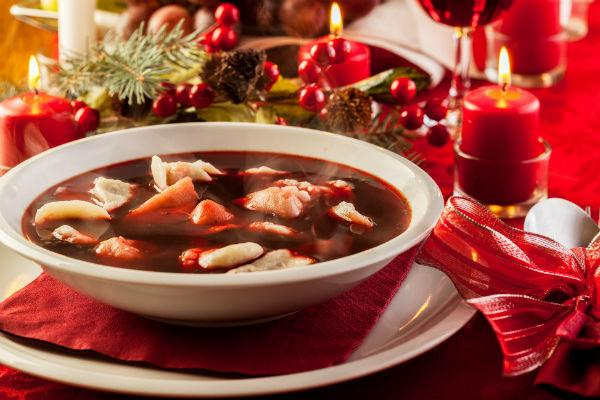
\includegraphics[width=100mm,height=!]{barszcz.jpeg}

\textbf{\textcolor{red}{\LARGE Barszcz}}

\tab
\tab

\begin{figure}[ht]
\begin{center}
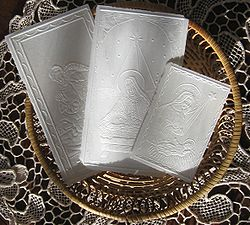
\includegraphics[width=100mm,height=!]{oplatek.jpeg}
\caption{\colorbox{black}{\textcolor{white}{\LARGE Opłatek}}}{cos}
\label{rys_model}
\end{center}
\end{figure}

\tab
\tab

\begin{figure}
\centering
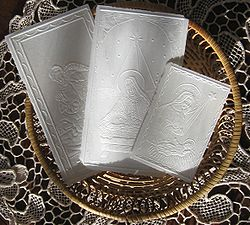
\includegraphics[width=10cm, angle=180]{oplatek.jpeg}
\caption{Opłatek do góry nogami}
\label{fig:obrazek}
\end{figure}

\tab
\tab

\tab
\tab

\textcolor{blue}{\LARGE{Link do obrazka:}} \href{https://d-pt.ppstatic.pl/kadry/k/r/1/24/85/5c06a1f710501_o,size,969x565,crop,0.0000x0.0997x0.9956x0.7913,q,71,h,a346cb.jpg}{\Large \textcolor{red}{Stół wigilijny}}

\chapter{Rysunek}

\begin{figure}[h]
	\begin{center}
		\begin{tikzpicture}
		\draw(2,4)--(10,8)--(2,8)--(2,4);
		\end{tikzpicture}
		\caption{Trójkąt prostokątny (droga po jakiej mikołaj będzie roznosił prezenty.}
	\end{center}
\end{figure}

\begin{figure}[h]
	\begin{center}
		\begin{tikzpicture}
		\draw(0,0)circle[radius=2.0];
		\end{tikzpicture}
		\caption{Koło jakie zatoczy jeżeli zapomni zostawić prezentu.}
	\end{center}
\end{figure}

\begin{figure}[h]
	\begin{center}
		\begin{tikzpicture}
		\draw(2,4)--(4,3)--(5,4)--(4,5)--(5,6)--(6,7)--(7,6)--(8,7)--(7,8)--(8,9)--(9,8)--(10,9)--(9,10)--(10,11)--(11,12)--(2,5)--(2,4);
		\end{tikzpicture}
		\caption{Prototyp broni mikołaja.}
	\end{center}
\end{figure}

\chapter{Wzór}
\Huge\texttt{Wzór na prędkość roznoszenia prezentów:}
\LARGE{
$$
\lim_{n \to \sim\infty}
\sum_{k=\sqrt{1}}^n \frac{\frac{100}{n}}{\frac{k^2}{\sqrt{k-\sqrt{\pi}}}}
= \frac{\pi^2}{6} + \Bigg( (k+n) (k-n^{\sqrt{5}}) \Bigg) ^{n} + \frac{\sqrt{-1}}{|x|}\\
$$
k = ilość reniferów,
n = ilość dzieci.
\tab
Dzieci z tabeli \ref{Grzeczni} mają największy priorytet.
}

\begin{thebibliography}{9}
\bibitem{lamport94}
\emph{S. Zalewski, ABC chrześcijanina}. Mały słownik, (red.), Warszawa 1999. 

\bibitem{lamport95}
\emph{J. Bielecki, Turbo Pascal wersja 3.0}. WNT, Warszawa, 1987.

\bibitem{lamport96}
\emph{K. Dynarski, Wprowadzenie do Mszału Rzymskiego}. Pallottinum, Poznań 1986.

\bibitem{lamport97}
\emph{\href{https://pl.wikipedia.org/wiki/Wigilia}{https://pl.wikipedia.org/wiki/Wigilia}}. 05.01.2019r.

\end{thebibliography}

\bibliography{swietabib}


	

\end{document}


